\begin{figure*}[t]
\centering
\subfigure[Evaluation results from the Support Vector Machine.] {
\includegraphics[width=\columnwidth]{precission-recall}
\label{fig:prediction-svm}
}
\subfigure[Evaluation results from the Logistic Regression.] {
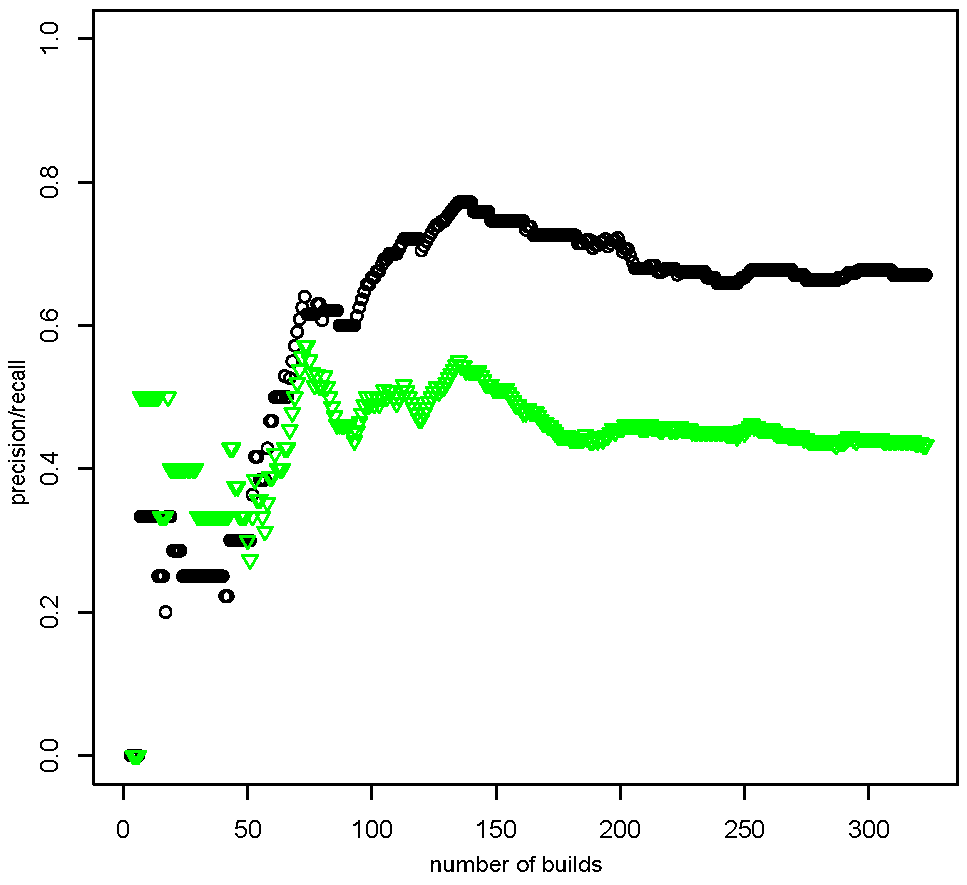
\includegraphics[width=\columnwidth]{precision-recall-logreg}
\label{fig:prediction-logreg}
}
\caption{Plotting the precision (green downward pointing triangles) and recall (black hollow circles) of the support vector machine (left) and the logistic regression (right).}
\label{fig:prediction}
\end{figure*}

\section{Build Failure Prediction}
\label{sec:prediction}
To answer our first research question, we build a predictive model that uses the
constructed socio-technical networks as input to predict whether a build succeeds
or fails. Since we are interested in the practical application of this model we
diverge from the standard evaluation tactic and use a more practical relevant
approach. After we presente the results of our prediction model we discuss their
implications.

\subsection{Model Evaluation}
We train several prediction models, such as logistic regression, support vector
machines, decision trees, and a bayesian classifiers, using features we
extract from the constructed socio-technical networks. Each feature represents a pair of
connected developers in the network and the type of the edge that they are
connected with (i.e. social, technical or socio-technical).

%To evaluate those model, we take a more practical evaluation approach.
To accomplish a more practical evaluation, we order all our social networks by the time the build they were constructed from was tested.
Having the networks ordered according to build time we evaluate our prediction model in the following five steps:%\todo{make pictures}

\begin{enumerate}
\item Get the first $n$ networks and perform a principle component analysis on the extracted features.
\item Select the principal components that explain the most variance until 95\% of the total variance of the training set can be explained.
%\item Determine the principal components of the first $n$ networks.
\item Train the model using the principal components of the first $n$ networks.
\item Test the model on network $n+1$ after transforming it to the determined principal components.
\item Increase $n$ by 1 and repeat until $n+1$ is the size of complete data set.
\end{enumerate}

This evaluation technique is meant to simulate the actual usage of the prediction model.
In software practice builds come in one by one.
This means that whenever a build has been verified the model can be extended using the social network from the newest build for training. 
This method of evaluation is closer to the actual usage in the field than
random splits or cross validation.

We used two coefficients to assess the models quality at any given time: recall (Eq.~\ref{eq:recall}) and precision (Eq.~\ref{eq:precision}).
The recall of a model describes the percentage of how many failed builds where predicted correctly.
This translates into the formula:

\begin{equation}
\label{eq:recall}
\text{recall}=\frac{\text{Correctly \emph{as failed} Predicted Builds}}{\text{All Failed Builds}}
\end{equation}

Precision on the other hand describes the percentage of how many of the \emph{as failed} predicted builds are actually failed builds. Thus we can express precision using the following formula:

\begin{equation}
\label{eq:precision}
\text{precision}=\frac{\text{Correctly \emph{as failed} Predicted Builds}}{\text{All \emph{as failed} Predicted Builds}}
\end{equation}

Both recall and precision lie in the interval from 0 to 1, with 1 being best and 0 being worst.
We compute the recall and precision for each iteration by accumulating the prediction results of all previous prediction results.
For example if we went through 20 iterations we create a contingency table from the predicted results for the last 20 builds.
Each prediction can have one of four outcomes: (1) correctly predicted \emph{as failed}, (2) correctly predicted as succeeded, (3) falsely predicted \emph{as failed}, and (4) falsely predicted as succeeded.
Adding those numbers till the most recent prediction enables us to compute precision and recall.


The current standard evaluation for failure prediction models in software engineering is to take the data set and generate a number of random splits (e.g.~\cite{zimmermann:icse:2008,schroeter:isese:2006,nagappan:icse:2008}).
A random split partitions the data into a training and a testing data set, where the model is trained with the training data and then evaluated using the testing set.
Other also used cross validation which creates $n$ partitions and tests with each partition while training with the remaining $n-1$ partitions (e.g.~\cite{wolf:icse:2009}).

Although random splits and cross validation allow for a random combination, they completely ignore the explicit order.
This leads to the problem that random splits and cross validation allow features that might emerge later and should not have been available to be used for training.
For example, if a developer joins the project after it started, she cannot have been present in any of the networks previous to her date of joining the project.
This means that the model at first cannot use any information about her connections to others.

%%%%%%%%%%%%%%%%%%%%%%%%%%%%%%%



\subsection{Results}
Of the prediction models we evaluated, we present the results for the support
vector machine and the logistical regression. The support vector machine produced
the best results whereas the logistical regression serves as comparison to the
support vector machine results as well as indicating the reliability of
the regression analysis presented later in Section~\ref{sec:pattern}.

% describe support vector machine \todo{talk about three sections of the figures}
Figure~\ref{fig:prediction} shows the recall and precision values for the
suport vector machine and the logistical regression models. The green downward
pointing triangles represent the precision of the model for each iteration, note that we started training each model with at least three data points. The black circles represent the recall of a model for each
iteration.

Both Subfigures in Figure~\ref{fig:prediction} can be divided into three
sections. The first section is comprised of the first 70-80 iterations where,
by a manual investigation, we observe that the support vector machine predicts almost everything to be successful in contrast to the unstable logistic regression.

The middle section is characterized by a peek efficiency between 100 and 150
iterations in both prediction models. Before that peak both models underperform, where the support vector machine suffers more than the logistic regression from a small data set.

In the last segment after 150-180 iteration the precision and recall values
stabilize over both models. In contrast to the logistic regression the support vector machine obtains a higher precision and a lower recall with a slight upward trend.
The support vector machine ended with a precision of $.68$ (median: $.67$) and a recall of $.49$ (median: $.45$) whereas the logistic regression obtained a precision and recall value of $.43$ (median: $.45$) and $.67$ (median: $.67$) respectively.












\subsection{Discussion}
% - why did we fulfill our objective
Although the overall performance of the models is not yet practical due to low
precision and recall, these results are interesting. On the one hand, we consider
answering our first research question with yes: we can use developer pairs to
predict build failure. We consider the model to be sufficient because we, as Wolf
et al.~\cite{wolf:icse:2009}, outperform a random guess which would have
resulted in both recall and precision of less than $.33$, which is the percentage of failed
builds. To our knowledge there have been only two studies that focused on
predicting build outcomes: by Hassan et al.~\cite{hassan:ase:2006} and by Wolf et
al.~\cite{wolf:icse:2009}. Our approach places itself between the results of both
studies with our study being better than results obtained by Wolf et
al.~\cite{wolf:icse:2009} but being worse than Hassans et
al.~\cite{hassan:ase:2006} approach.

Despite of outperforming the random guess the precision of our models is of concern because
it indicates the rate at which we falsely report a build to fail. With a median
 precision of $.67$, every third of the \emph{as failed} build predicted by the support
 vector machine would be a false positive. Besides the low trust a developer
 can develop in the model, it also reports less than half of the failed builds
 as failed.


% - why is the beginning so weak
We provide some possible explanations here. In the first part of the
Figures~\ref{fig:prediction-svm} and~\ref{fig:prediction-logreg}, we observed
that all models perform poorly as long as they have less than 100 builds to train
on. After investigating the first 100 builds we found that new
developers are continually appearing in the development pairs. This means that
prediction models need to make predictions without having enough knowledge to
train on, thus resorting to predict the build to be the most likely outcome, to be OK.

%- check peeks with respect to new developers entering the team
A peak in the interval of 100-150 iterations occurred in both models for both recall and precision.
Within this interval the team changed and new people joined the project and people where reallocated to work on new functionality which meant creating new dependencies and leaving old dependencies behind.
This change in dependencies confused the model in a way that it did not perform as well.
Both models stabilize over time with the support vector machine exhibiting a slight upward trend.

% - what is the next step
Since the goal of this research is to find a way to create actionable knowledge
to avoid build failure, building a prediction model was the first step to show
that developer pairs have an effect on the actual prediction. The results from
the prediction models is first evidence that developer relationships have an
influence on the build. Next we continue with perusing our second research
question that examined the relationship between particular developer
pairs (i.e. technical pairs) and build results. This will help us
investigate how we might prevent builds from failing by changing the
nature of developer relations in these pairs.



